% The finned-tube device: a section along the tubes and a section across them
\documentclass[tikz, border=4pt]{standalone}
% Shared preamble of the PyTES model diagrams: packages, colours and styles.
% Each diagram is a standalone document that inputs this file; build them with build.py.
\usepackage{amsmath}
\usepackage{bm}
\usetikzlibrary{arrows.meta, calc, decorations.pathreplacing, patterns, positioning}

% The PyTES Thermal colour cycle (pytes.plotting.THERMAL) and tints of it
\definecolor{pytesorange}{HTML}{E8590C}
\definecolor{pytesblue}{HTML}{1F4E9C}
\definecolor{pytesteal}{HTML}{14A08A}
\definecolor{pytesamber}{HTML}{F0A930}
\definecolor{pytesplum}{HTML}{A23B72}
\definecolor{pytessky}{HTML}{88C7F0}
\definecolor{pytesink}{HTML}{36312E}

% Materials: the heat transfer fluid, the PCM, the metal (fins and tubes)
\colorlet{fluidfill}{pytessky!75}
\colorlet{pcmfill}{pytesamber!55}
\colorlet{liquidfill}{pytesorange!60}
\colorlet{metalfill}{pytesink!45}
\colorlet{compositefill}{pcmfill!85!metalfill}

\tikzset{
  >={Stealth[length=2.2mm]},
  every picture/.style={line join=round, line cap=round, font=\small},
  outline/.style={draw=pytesink, line width=0.6pt},
  fluid/.style={outline, fill=fluidfill},
  pcm/.style={outline, fill=pcmfill},
  liquid/.style={outline, fill=liquidfill},
  metal/.style={outline, fill=metalfill},
  composite/.style={outline, fill=compositefill},
  flow/.style={->, draw=pytesblue, line width=1.2pt},
  heat/.style={->, draw=pytesorange, line width=1.1pt},
  axis/.style={->, draw=pytesink, line width=0.7pt},
  dimension/.style={<->, >={Stealth[length=1.6mm]}, draw=pytesink, line width=0.5pt},
  guide/.style={draw=pytesink!60, line width=0.4pt, dashed},
  symmetry/.style={draw=pytesink, line width=0.5pt, dash dot},
  label/.style={text=pytesink, font=\small},
  note/.style={text=pytesink, font=\footnotesize, align=center},
}

\begin{document}
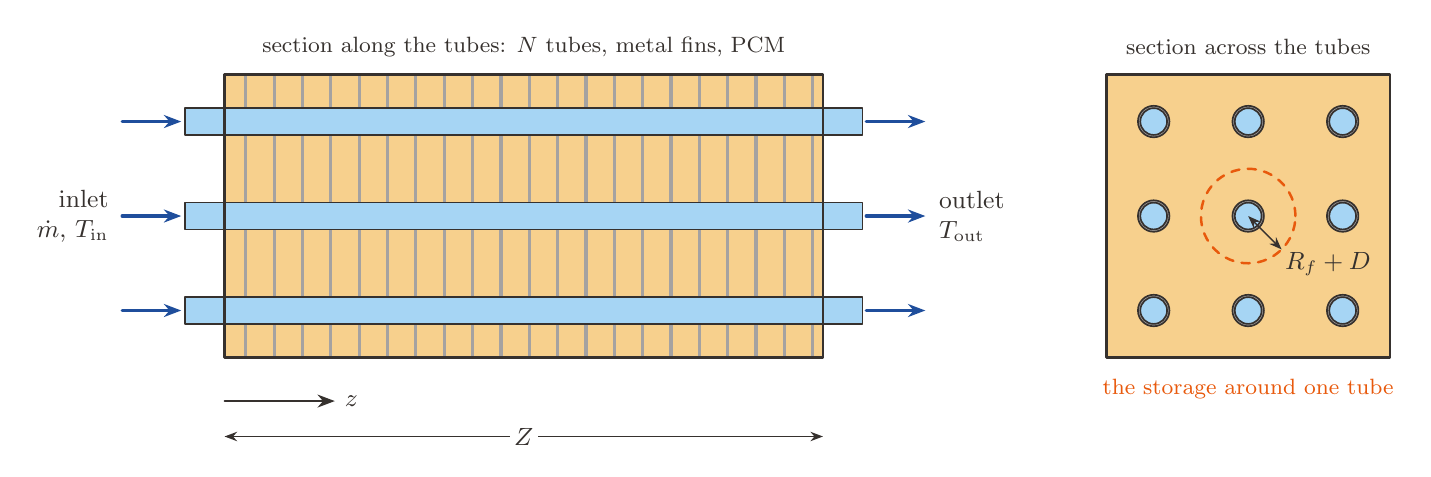
\begin{tikzpicture}
  % (a) Section along the tubes
  \begin{scope}
    \def\L{7.6}
    \def\Hb{3.6}
    \fill[pcmfill] (0, 0) rectangle (\L, \Hb);
    \foreach \i in {0, ..., 20} {
      \fill[metalfill] ({0.25 + 0.36*\i}, 0) rectangle ({0.29 + 0.36*\i}, \Hb);
    }
    \foreach \yc in {0.6, 1.8, 3.0} {
      \draw[fluid] (-0.5, \yc - 0.17) rectangle (\L + 0.5, \yc + 0.17);
      \draw[flow] (-1.3, \yc) -- (-0.55, \yc);
      \draw[flow] (\L + 0.55, \yc) -- (\L + 1.3, \yc);
    }
    \draw[outline, line width=1pt] (0, 0) rectangle (\L, \Hb);
    \node[label, anchor=east, align=right] at (-1.35, 1.8) {inlet\\$\dot m$, $T_\mathrm{in}$};
    \node[label, anchor=west, align=left] at (\L + 1.35, 1.8) {outlet\\$T_\mathrm{out}$};
    \draw[axis] (0, -0.55) -- (1.4, -0.55) node[label, right] {$z$};
    \draw[dimension] (0, -1.0) -- (\L, -1.0) node[label, midway, fill=white, inner sep=1.5pt] {$Z$};
    \node[note] at (\L/2, \Hb + 0.35) {section along the tubes: $N$ tubes, metal fins, PCM};
  \end{scope}
  % (b) Section across the tubes, between two fins
  \begin{scope}[shift={(11.2, 0)}]
    \def\s{1.2}
    \fill[pcmfill] (0, 0) rectangle (3*\s, 3*\s);
    \foreach \i in {0, 1, 2} {
      \foreach \j in {0, 1, 2} {
        \draw[metal] ({(\i + 0.5)*\s}, {(\j + 0.5)*\s}) circle (0.2);
        \draw[fluid] ({(\i + 0.5)*\s}, {(\j + 0.5)*\s}) circle (0.17);
      }
    }
    \draw[outline, line width=1pt] (0, 0) rectangle (3*\s, 3*\s);
    \draw[pytesorange, line width=0.9pt, dashed] (1.5*\s, 1.5*\s) circle (0.5*\s);
    \draw[dimension] (1.5*\s, 1.5*\s) -- ++(-45:0.5*\s)
      node[label, pos=1, below right, inner sep=1pt] {$R_f + D$};
    \node[note, text=pytesorange, anchor=north] at (1.5*\s, -0.15)
      {the storage around one tube};
    \node[note] at (1.5*\s, 3*\s + 0.35) {section across the tubes};
  \end{scope}
\end{tikzpicture}
\end{document}
